\chapter{System Maintenance}

\section{Environment}

\subsection{Software}

The following is the software used during my implementation.

\begin{itemize}
\item Python 3.3 and 3.4
\item IDLE
\item PyQt 4
\item SQLite 3
\item SQLite Inspector
\item SQLite Database Browser
\item Matplotlib
\item Adobe Photoshop CS5
\end{itemize}

\subsection{Usage Explanation}

\begin{center}
    \begin{tabular}{|p{4cm}|p{6cm}|}
        \hline
        \textbf{Test Series} & \textbf{Purpose of Test Series} \\ \hline
        Python 3.3 and 3.4 & Used as my programming language to produce my system. I have chosen this language as I have been learning it in class for the past two years \\ \hline
        IDLE & I used this software as the developing environment. It was included with Python and has been the environment I have been using in classes so I am familiar with it. This made implementation easier\\ \hline
        PyQt 4 & Used to create the graphical user interface for my program \\ \hline
        SQLite 3 & This was used to access my database in order to extract and store information \\ \hline
        SQLite Inspector & This software allowed me to browse the database file when implementing the system. It was used to check data was being added, removed and changed correctly if accessed from inside the system. \\ \hline
        SQLite Database Browser & This program is similar to the inspector but was downloaded when I was working on my Macbook (rather than my computer). It performs the exact same task of viewing data in the database file. \\ \hline
        Matplotlib & This allows for extracting data from the database to produce graphs \\ \hline
        Adobe Photoshop CS5 & Used for creating the splash screen and adding transparency to arrows \\ \hline
    \end{tabular}
\end{center}

Python features allowed me to run my system which let me
implement and test my system in a CLI or GUI form. This will
be used to run my system in its GUI form for my client.

\subsection{Features Used}

\begin{center}
    \begin{tabular}{|p{4cm}|p{6cm}|}
        \hline
        \textbf{Test Series} & \textbf{Purpose of Test Series} \\ \hline
        Python 3.3 and 3.4 & Python provided me with the features needed to create my program in both CLI and GUI form. Python allows modules to be imported from elsewhere such as matplotlib (see below).  \\ \hline
        IDLE & IDLE is an environment specifically for Python and was used to create and run the code. The syntax highlighting that IDLE uses made implementing the program easier. \\ \hline
        PyQt 4 & A lot of features were used of PyQt such as stacked widgets, main windows and widgets. \\ \hline
        SQLite 3 & SQLite3 is essentially a simplified version of MySQL and included all of the functions I needed to deal with databases in my system. One of the features that was especially important was enforcing referential integrity which ensured that foreign keys matched existing primary keys.  \\ \hline
        SQLite Inspector & The execute feature was used to debug my SQL, this allowed me to test queries before they were ran in Python  \\ \hline
        SQLite Database Browser & I used this program for the same features as the Inspector shown above.   \\ \hline
        Matplotlib & The module from marplotlib known as 'Pylab' was used to create my graph, more specifically it was used to create a bar chart with axes titles.  \\ \hline
        Adobe Photoshop CS5 & The magic wand tool was used to remove image backgrounds (making them transparent), layering and selection tools were also used to create and edit images. \\ \hline
    \end{tabular}
\end{center}

\section{System Overview}

\subsection{Logins}

This part of the system will prevent any unauthorised access to the system. It will check the username and password input and compare it with usernames and passwords stored in a database file. If the details match the user will gain access to the relevant part of the system. The system runs with access restrictions therefore usernames will have certain access levels attached to them which are (in order of access rights) Admin, Manager or Staff. If the username/password combination does not match a error will appear asking the user to re-enter the information until it is correct. There is also a "forgotten username or password" button to allow users to send emails to IT staff from inside the system which will request a password retrieval.

\subsection{The Graphical User Interface}

The whole system is built with a graphical user interface (GUI) to make sure it is professional and user friendly. The GUI contains many different features including:
\begin{itemize}
\item Toolbar icons and menu bars for navigational purposes
\item Images to improve to overall look of the system
\item File browsing to choose the database
\item Line edits and combo boxes to allow a user friendly input of data
\item Labels for certain parts of the system to tell users what interface they are currently viewing
\item Stylesheets to improve the overall look and to match company website colours
\end{itemize}

\subsection{Open Database Interface}

The admin main menu will provide a button that will take the user to the 'Open Database' interface. This will most likely be the most used interface on the entire system because this is where IT Staff can add, remove and edit records on the database. The user can choose the database file from a file browsing window and view each table using a combo box. After a table is selected the user can then use the buttons on screen to remove, add or edit. Removing data will allow the user to delete an entire record from the click of a button, the edit button will allow the user to simply edit the cell contents and save changes afterwards. The add button will take the user to another window to add data to the database (see below)

\subsection{Adding Data}

Adding data is done only from the admin interface. Depending on which table is being viewed on the 'Open Database Interface' (see above) when the user clicks the 'Add Data' button, input fields for the specified table will appear in a dialog box. The user can then enter information into the line edits, validation is used to make sure the correct data is being entered. If the wrong data is entered into a field an error message will appear as the placeholder text for the specified field. After the user has finished the data will be added into the database.

\subsection{Searching Staff}

Another important part of the system on the admin interface is the search staff interface, this allows the user to search for staff members by department. Each department will be shown in a combo box and to search for a staff member the user will enter a first name into the search box. After the correct staff member has been found the user may click on a labelled button to view more information about which hardware devices they own.

\subsection{Graph Representation}

A graph can be generated through a toolbar button on the admin user interface. This is used as a clear representation of how many hardware devices are owned by each department in a bar chart format. The graph is populated by looking at how many staff members own hardware (and how many they own), then recording which department they are from.

\subsection{Department Information for Managers}

The manager interface allows them to view staff information from their own department. Managers will only be able to view one table from the database which will tell them which hardware devices the staff own along with the purchase date. 

\subsection{Personal Information}

Managers and other staff members are able to view their own information which will display the hardware devices they own, they can then check for any errors in the information or use it to provide proof of purchase. Staff members (not admins or managers) only have access to this one interface and cannot check anyone else's information due to the access restrictions. Search bars are in place incase the table gets highly populated. This part of the system will most likely be used the least as it is only in place for convenience to view hardware, it will not be used on a daily basis.

\subsection{Adding Accounts}

To use the login system correctly user accounts need to be made. IT staff can create user accounts using the toolbar button on the admin interface. To initially access the system I will provide a default username/password to my client that they can then change later on. The account creation interface allows IT staff to enter a first name and last name, department and access rights. The program will then automatically generate the account details, the username will be generated by taking the first name initial along with the last name and adding a random integer up to 20 to the end. The password is made by randomly generating upper and lowercase letters and numbers with a length of 7 characters. The user can generate as many different combinations as they want or enter the account details manually.

\section{Code Structure}

My code was split into different files for each different main functionality or class. This is because it allowed me to work on each part of the system individually and located specific areas easily.

%use as many subsections as necessary for the code sections
\subsection{Admin - Main Window}
%the code below can be uncommented and used to get a code section from a particular file
\begin{figure}[H]
    \pythonfile[firstline=17,lastline=41]{./Implementation/Files/MainProgram.py}
    \caption{The program has three Main Window classes that will be used to import other widgets into them. These widgets can then be added to a stack so switching between interfaces can be done easily. The above class is to control the admin interfaces. A class was chosen with methods so that functions can be grouped together. Classes can then inherit from each other so that no code is unnecessarily repeated.} \label{fig:MainWindowAdmin}
\end{figure}

\newpage

\subsection{Dialog Box Class}
With the use of classes I can create instances of these classes from different functions whenever I wish to call them. For example the Presence Dialog class needs a text string so that specific text can be displayed on the warning.
\begin{figure}[H]
    \pythonfile[firstline=5,lastline=23]{./Implementation/Files/PopupDialog.py}
    \caption{This code section is the Presence Dialog class} \label{fig:Dialog Class}
\end{figure}

\begin{figure}[H]
    \pythonfile[firstline=465,lastline=468]{./Implementation/Files/OpenDatabaseWindow.py}
    \caption{This code section shows how a method is instantiating the class 'presence dialog class' with the specified text shown on line 2} \label{fig:Dialog Class}
\end{figure}

\subsection{Manager Menu Bar}

Menu bars are used on every interface in the system, therefore it was important to create menubar classes that can be reused in different parts of the system which avoids repeating code unnecessarily.  

\begin{figure}[H]
    \pythonfile[firstline=5,lastline=32]{./Implementation/Files/ManagerMenuBar.py}
    \caption{The above example is the Manager's menu bar that shows a menubar class, it can be called wherever needed.} \label{fig:Dialog Class}
\end{figure}

\begin{figure}[H]
    \pythonfile[firstline=84,lastline=86]{./Implementation/Files/ManagerMainProgram.py}
    \caption{This above example shows how to menubar is called.} \label{fig:Dialog Class}
\end{figure}

\subsection{Module Main Function}
 
 \begin{figure}[H]
    \pythonfile[firstline=286,lastline=291]{./Implementation/Files/MainProgram.py}
    \caption{Mostly all of my modules have this main function at the end of them, this allows me to test each modules individually to identify if it is working correctly and to test any bugs. With the specific example above the module takes a parameter when it is instantiated therefore it was important to include the None type in order to avoid errors.} \label{fig:Dialog Class}
\end{figure}

\section{Variable Listing}

\section{System Evidence}

\subsection{User Interface}


\begin{figure}[H]
    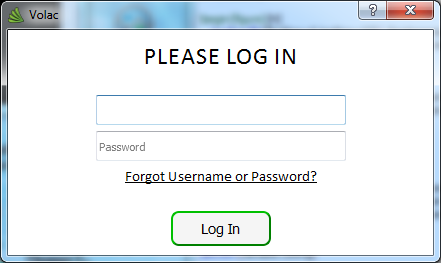
\includegraphics[width=\textwidth]{./Maintenance/Images/LoginWindow.png}
    \caption{The login screen that is displayed on initial startup.} \label{fig:LoginWindow}
\end{figure}

\begin{figure}[H]
    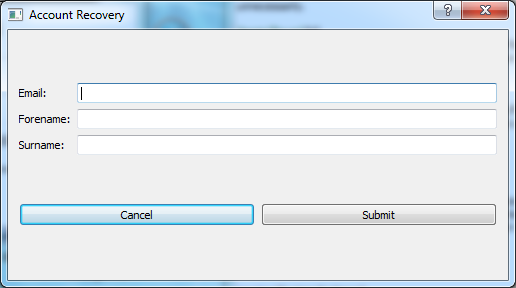
\includegraphics[width=\textwidth]{./Maintenance/Images/AccountRecovery.png}
    \caption{Account recovery window if the "forgotten username or password" button is clicked} \label{fig:AccountRecovery}
\end{figure}

\begin{figure}[H]
    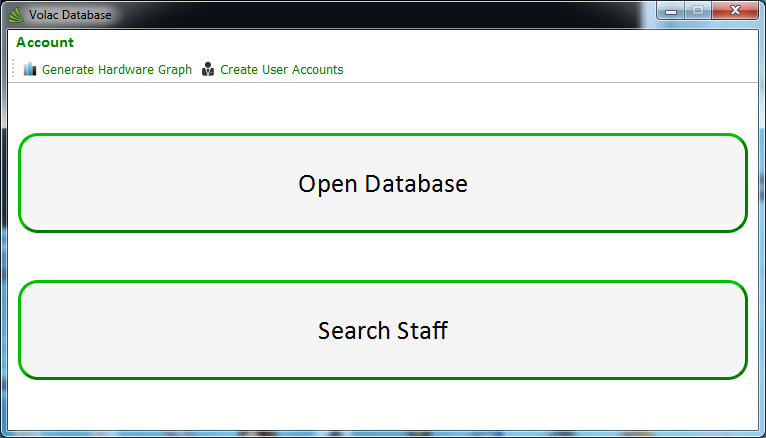
\includegraphics[width=\textwidth]{./Maintenance/Images/adminmainmenu.png}
    \caption{Admin main menu interface after log in} \label{fig:adminmainmenu}
\end{figure}

\begin{figure}[H]
    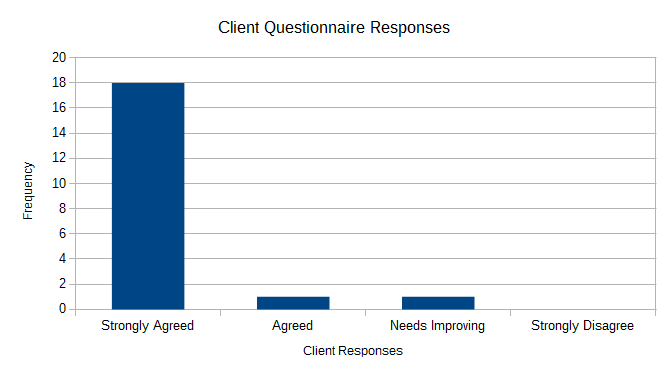
\includegraphics[width=\textwidth]{./Maintenance/Images/graph.png}
    \caption{Graph output showing departments number of hardware devices, activated when toolbar button is clicked} \label{fig:graph}
\end{figure}

\begin{figure}[H]
    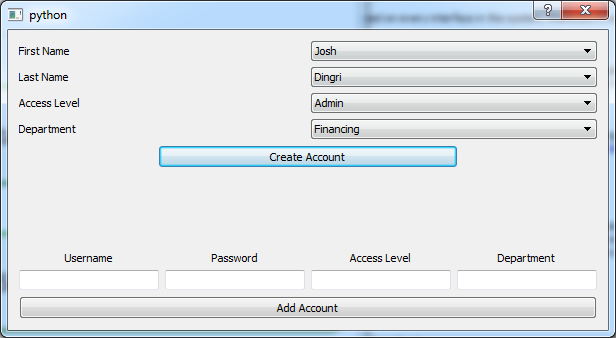
\includegraphics[width=\textwidth]{./Maintenance/Images/createaccounts.png}
    \caption{Create accounts window activated when toolbar button is clicked} \label{fig:createaccounts}
\end{figure}

\begin{figure}[H]
    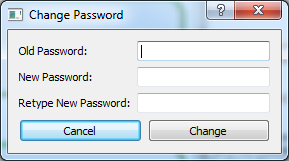
\includegraphics[width=\textwidth]{./Maintenance/Images/changepassword.png}
    \caption{Change password window activated when toolbar button is clicked} \label{fig:changepassword}
\end{figure}

\begin{figure}[H]
    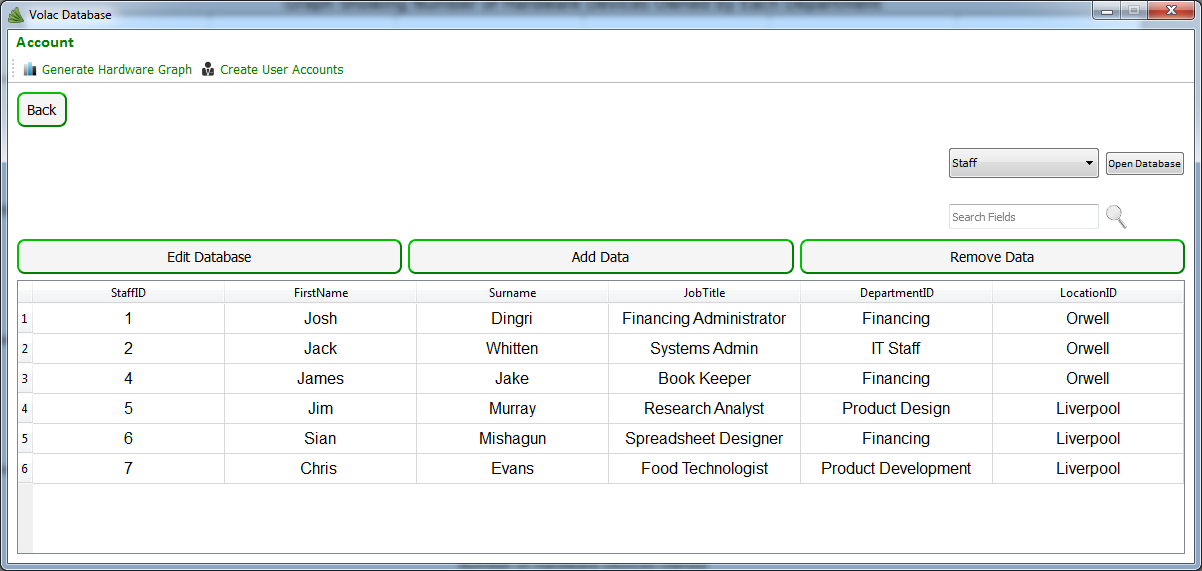
\includegraphics[width=\textwidth]{./Maintenance/Images/opendb.png}
    \caption{Open database interface, shown when user clicks button on the main menu} \label{fig:opendb}
\end{figure}

\begin{figure}[H]
    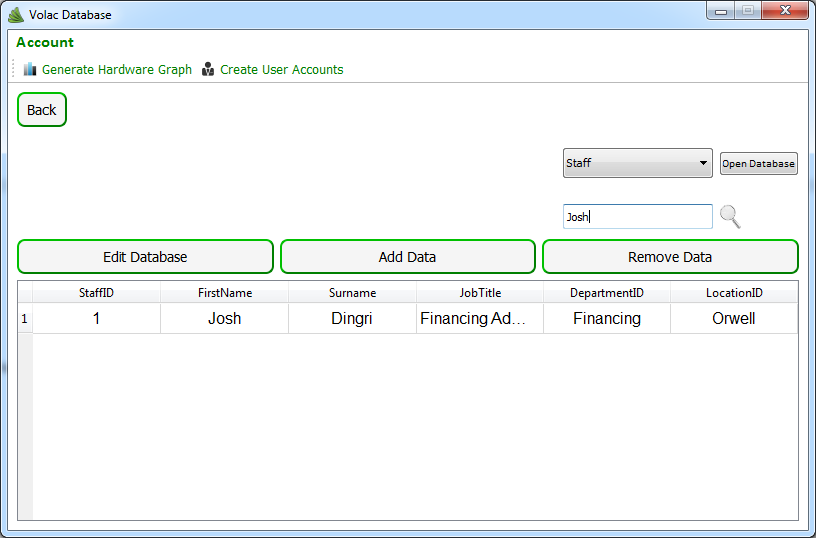
\includegraphics[width=\textwidth]{./Maintenance/Images/Searched.png}
    \caption{Result after text is entered into the search box} \label{fig:Searched}
\end{figure}

\begin{figure}[H]
    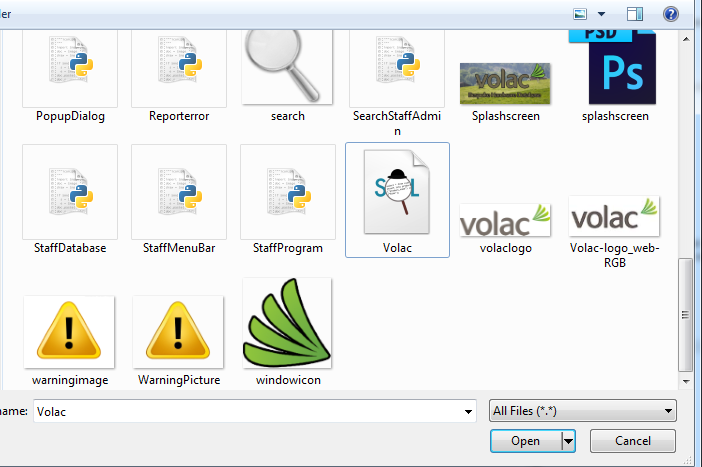
\includegraphics[width=\textwidth]{./Maintenance/Images/filebrowser.png}
    \caption{File browser to allow the user to choose the database file} \label{fig:filebrowser}
\end{figure}

\begin{figure}[H]
    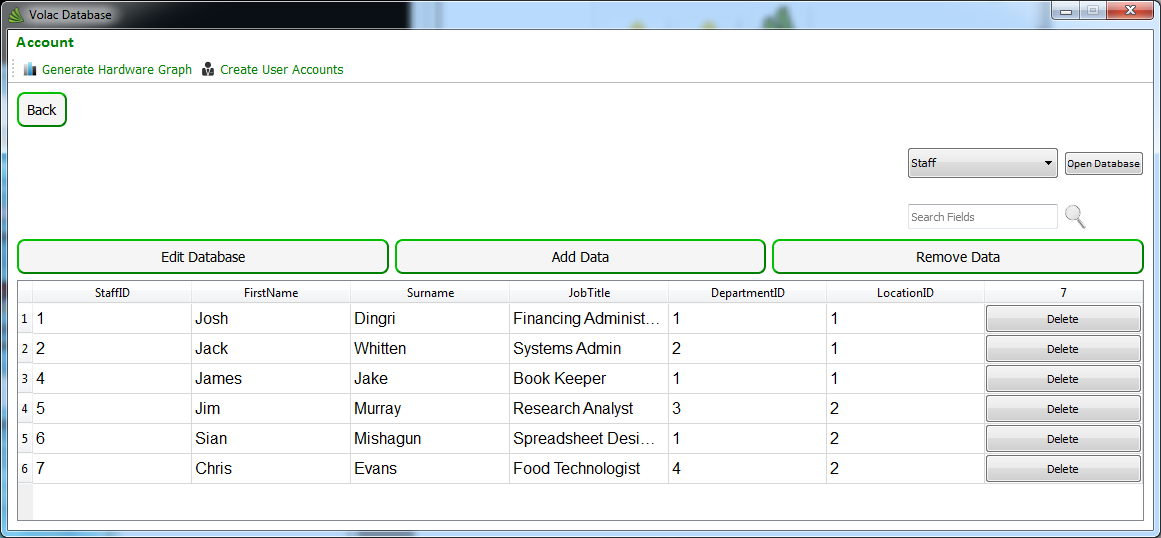
\includegraphics[width=\textwidth]{./Maintenance/Images/deletingdata.png}
    \caption{Delete buttons shown when the remove data button is pressed} \label{fig:deletingdata}
\end{figure}

\begin{figure}[H]
    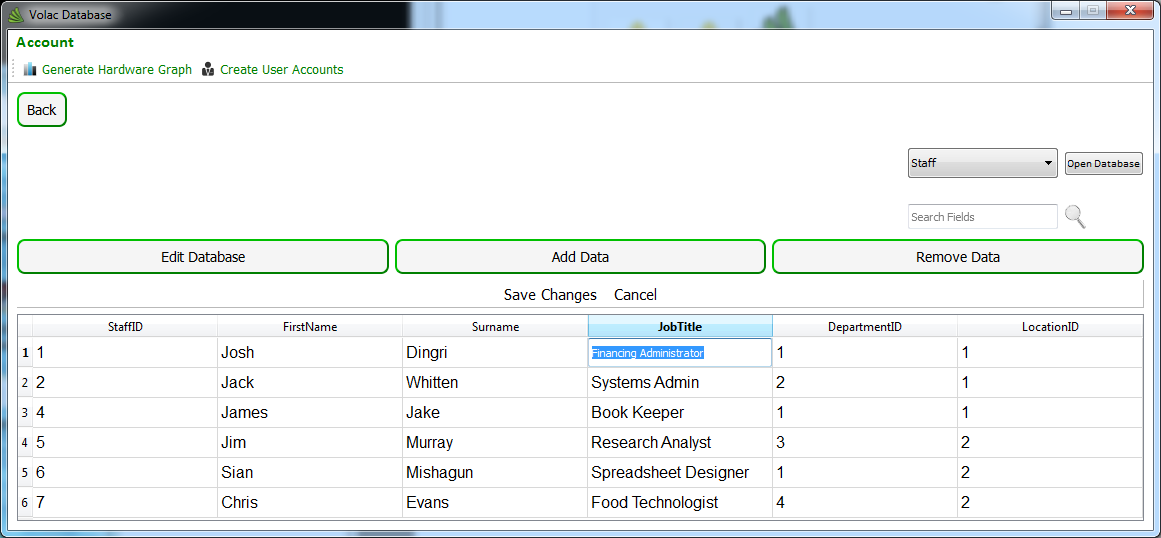
\includegraphics[width=\textwidth]{./Maintenance/Images/EditingData.png}
    \caption{User can edit data when edit data button is pressed} \label{fig:EditingData}
\end{figure}

\begin{figure}[H]
    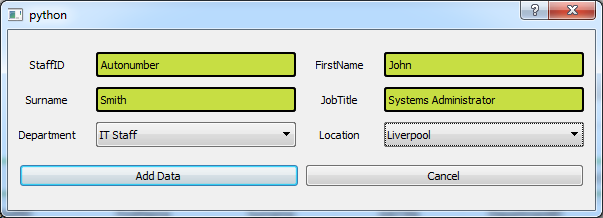
\includegraphics[width=\textwidth]{./Maintenance/Images/AddingData.png}
    \caption{The add data window to add data to the database.} \label{fig:AddingData}
\end{figure}

\begin{figure}[H]
    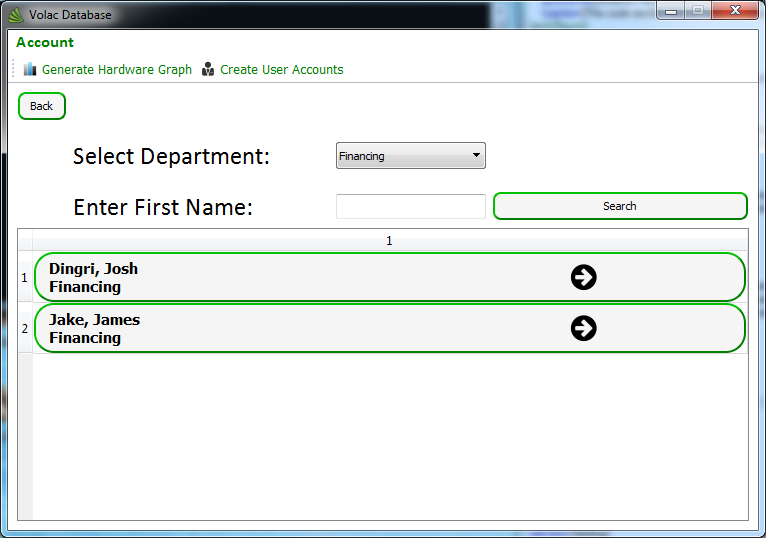
\includegraphics[width=\textwidth]{./Maintenance/Images/searchstaff.png}
    \caption{Search staff interface to search staff by department} \label{fig:searchstaff}
\end{figure}

\begin{figure}[H]
    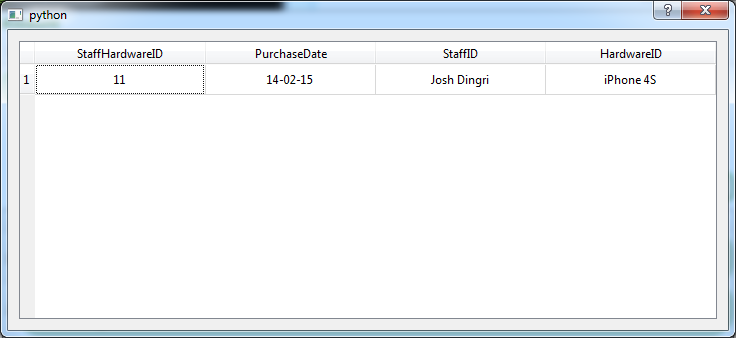
\includegraphics[width=\textwidth]{./Maintenance/Images/searchstaffresult.png}
    \caption{Window showing more information when a staff member is clicked on the search staff screen} \label{fig:searchstaffresult}
\end{figure}

\begin{figure}[H]
    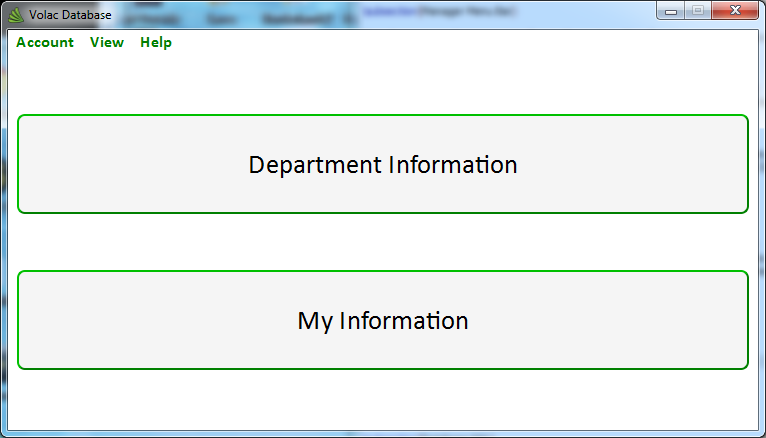
\includegraphics[width=\textwidth]{./Maintenance/Images/ManagerMM.png}
    \caption{Manager main menu after log in} \label{fig:ManagerMM}
\end{figure}

\begin{figure}[H]
    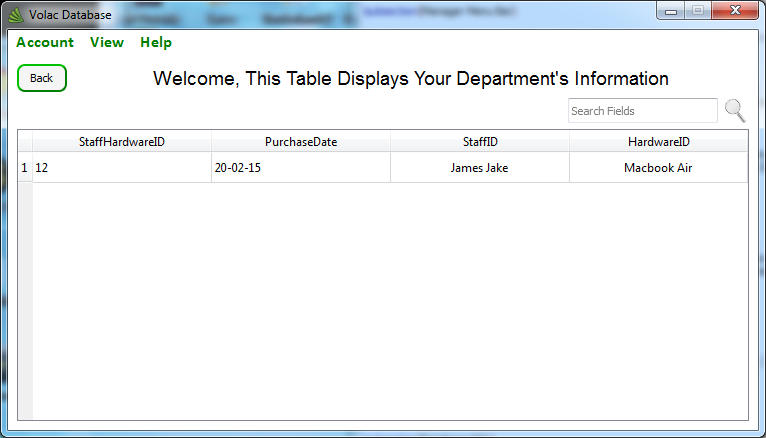
\includegraphics[width=\textwidth]{./Maintenance/Images/departinfo.png}
    \caption{Department information on manager interface} \label{fig:departinfo}
\end{figure}

\begin{figure}[H]
    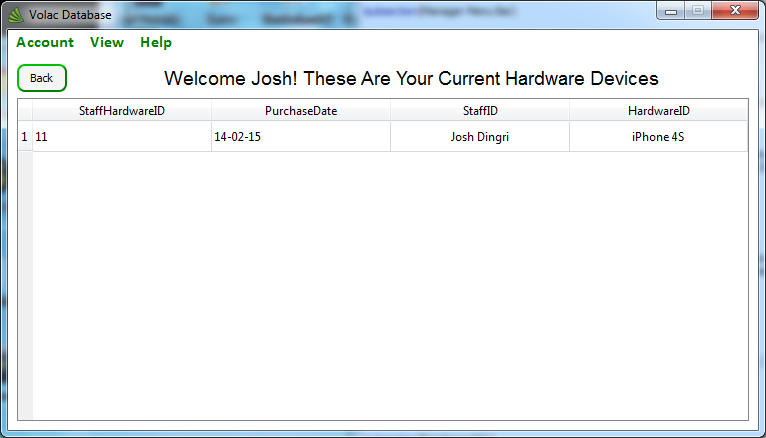
\includegraphics[width=\textwidth]{./Maintenance/Images/myinfomanager.png}
    \caption{Personal information ("My Information") interface shown for managers} \label{fig:myinfomanager}
\end{figure}

\begin{figure}[H]
    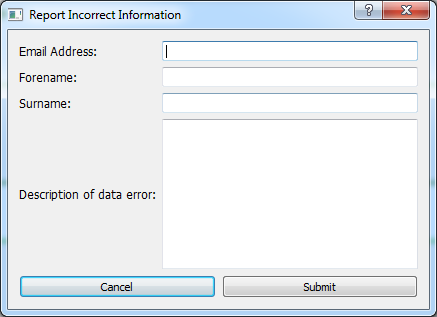
\includegraphics[width=\textwidth]{./Maintenance/Images/ReportError.png}
    \caption{The report errors email interface after toolbar button click} \label{fig:ReportError}
\end{figure}

\begin{figure}[H]
    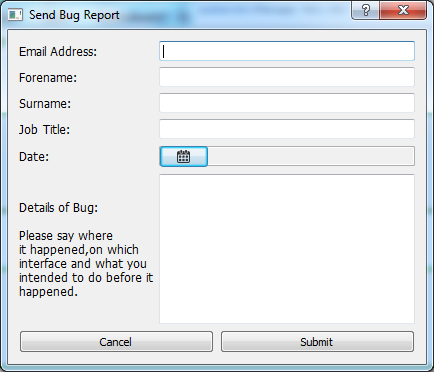
\includegraphics[width=\textwidth]{./Maintenance/Images/ReportBug.png}
    \caption{The report bug email interface after toolbar button click} \label{fig:ReportBug}
\end{figure}

\begin{figure}[H]
    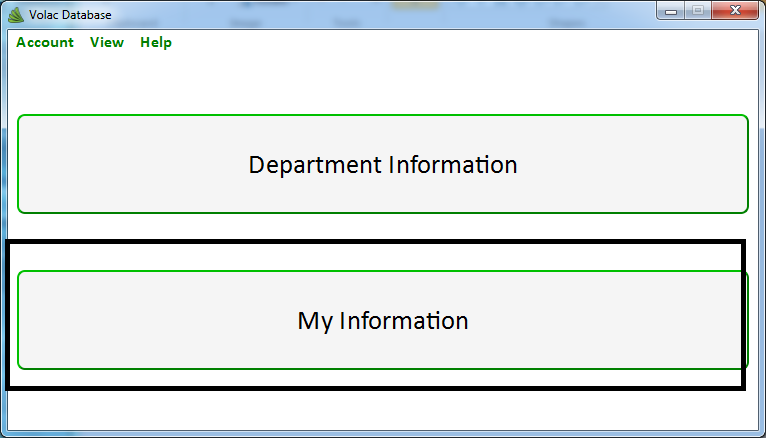
\includegraphics[width=\textwidth]{./Maintenance/Images/myinfo.png}
    \caption{Staff interface after login also showing personal information ("My Information") for staff} \label{fig:myinfo}
\end{figure}




\subsection{ER Diagram}

\begin{figure}[H]
    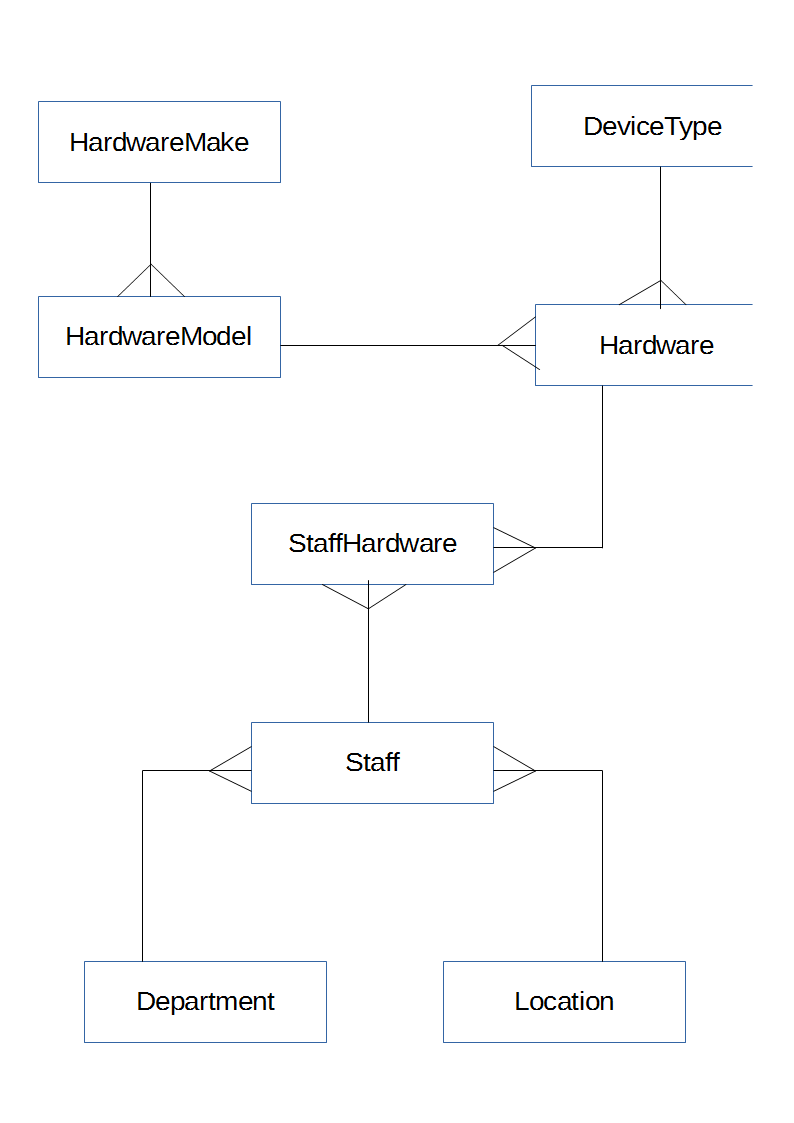
\includegraphics[width=\textwidth]{./Maintenance/Images/erupdateddiagram.png}
    \caption{Above is my final database which has been displayed as an Entity Relationship Diagram. It has changed slightly since my initial design.} \label{fig:erdiagram}
\end{figure}

\subsection{Database Table Views}

\begin{figure}[H]
    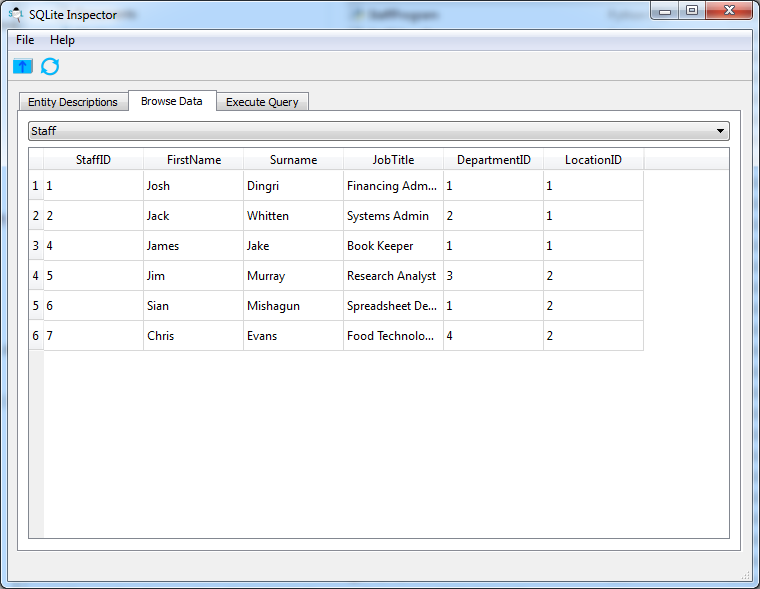
\includegraphics[width=\textwidth]{./Maintenance/Images/StaffTable.png}
    \caption{The "'Staff"' entity has 6 fields. The primary key of this entity is "StaffID". "DepartmentID" is a forein key that links to the "Department" entity (Fig: \ref{fig:DepartmentTable}) . "LocationID" is also a foreign key that links to the "Location" entity. (Fig: \ref{fig:LocationTable})} \label{fig:StaffTable}
\end{figure}

\begin{figure}[H]
    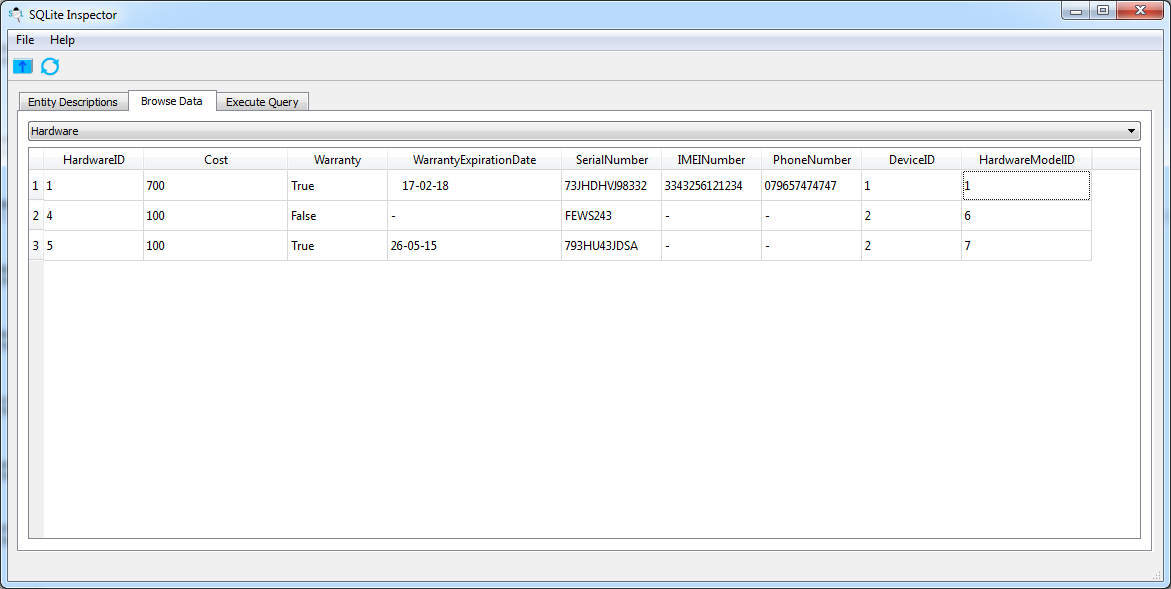
\includegraphics[width=\textwidth]{./Maintenance/Images/HardwareTable.png}
    \caption{The"Hardware" entity has 9 fields. The primary key of this entity is "HardwareID". "DeviceID" is a foreign key that links to the "DeviceType" entity  (Fig: \ref{fig:DeviceType}). "HardwareModelID" is also a foreign key that links to the "HardwareModel" entity (Fig: \ref{fig:HardwareModelTable})} \label{fig:HardwareTable}
\end{figure}

\begin{figure}[H]
    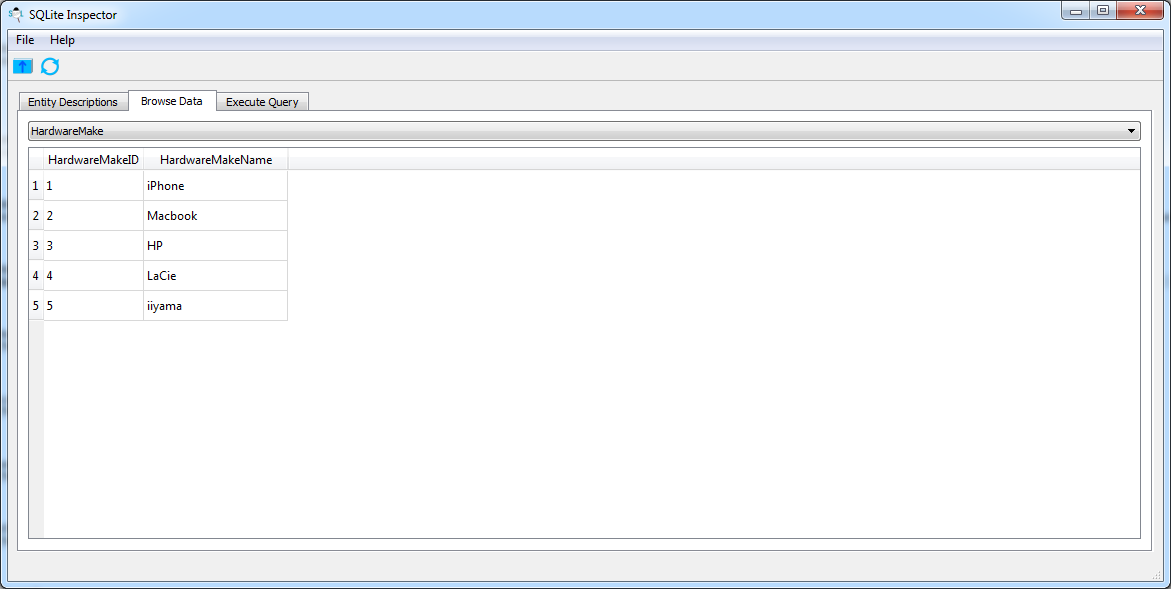
\includegraphics[width=\textwidth]{./Maintenance/Images/HardwareMakeTable.png}
    \caption{The "HardwareMake" entity has 2 fields. The primary key is "HardwareMakeID". The only store of data is the "HardwareMakeName" field} \label{fig:HardwareMakeTable}
\end{figure}

\begin{figure}[H]
    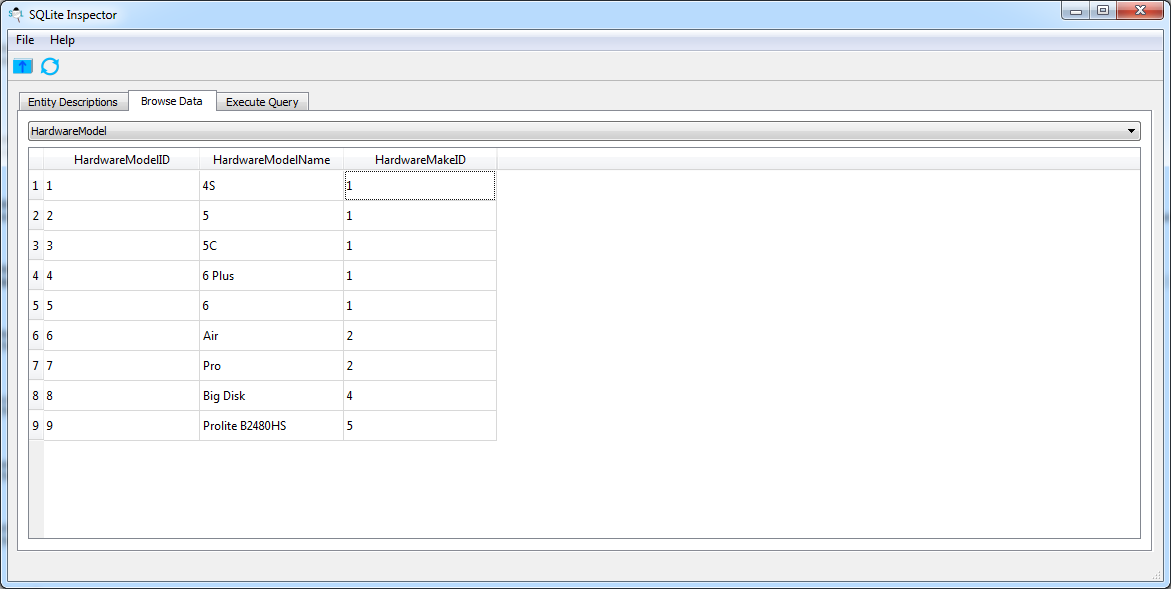
\includegraphics[width=\textwidth]{./Maintenance/Images/HardwareModelTable.png}
    \caption{The "HardwareModel" entity has 3 fields. The primary key is "HardwareModelID". The foreign key in this entity is "HardwareMakeID" which links to the "HardwareMake" entity. (Fig: \ref{fig:HardwareMakeTable})} \label{fig:HardwareModelTable}
\end{figure}

\begin{figure}[H]
    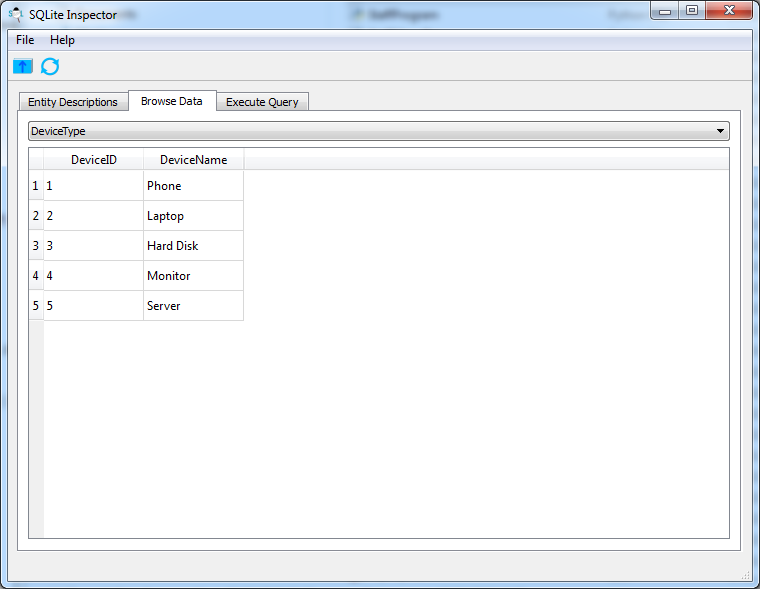
\includegraphics[width=\textwidth]{./Maintenance/Images/DeviceType.png}
    \caption{The "DeviceType" entity has 2 fields. The primary key is "DeviceID". The only store of data is the "DeviceName" field} \label{fig:DeviceType}
\end{figure}

\begin{figure}[H]
    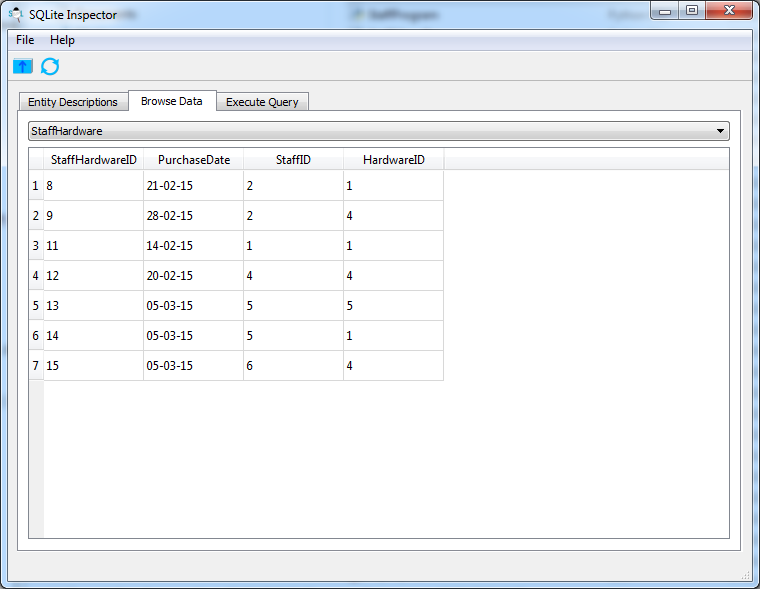
\includegraphics[width=\textwidth]{./Maintenance/Images/StaffHardware.png}
    \caption{The"StaffHardware" entity has 4 fields. The primary key of this entity is "StaffHardwareID". "StaffID" is a foreign key that links to the "Staff" entity  (Fig: \ref{fig:StaffTable}). "HardwareID" is also a foreign key that links to the "Hardware" entity (Fig: \ref{fig:HardwareTable})} \label{fig:StaffHardware}
\end{figure}

\begin{figure}[H]
    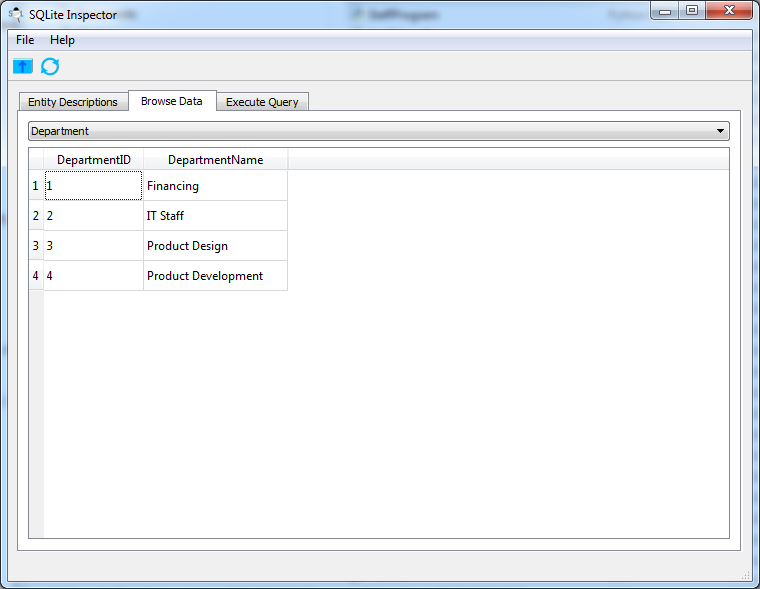
\includegraphics[width=\textwidth]{./Maintenance/Images/DepartmentTable.png}
    \caption{The "Department" entity has 2 fields. The primary key is "DepartmentID". The only store of data is the "DepartmentName" field} \label{fig:DepartmentTable}
\end{figure}

\begin{figure}[H]
    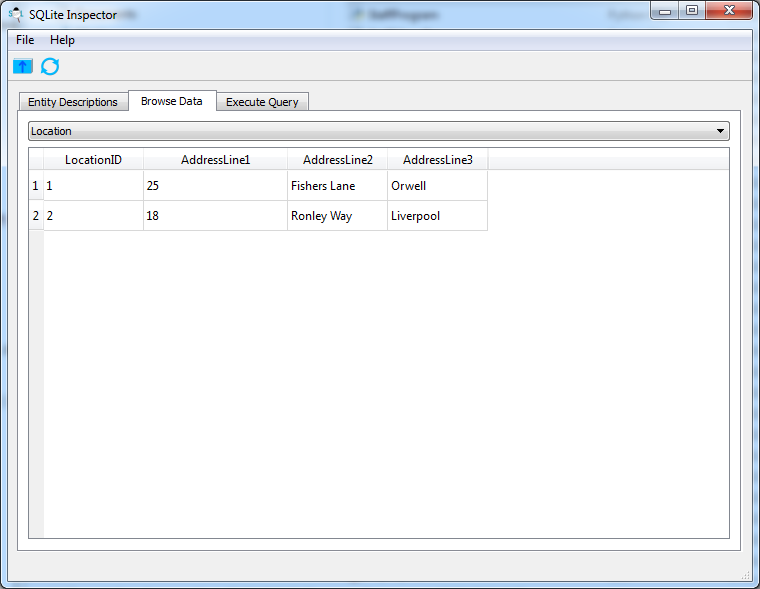
\includegraphics[width=\textwidth]{./Maintenance/Images/LocationTable.png}
    \caption{The "Location" entity has 4 fields. The primary key is "LocationID". The entity stores location details in the other 3 fields} \label{fig:LocationTable}
\end{figure}

\subsection{Database SQL}

The below is the SQL code which created each entity in the database.

\subsubsection{Staff Entity}

 \pythonfile[firstline=26,lastline=38]{./Implementation/Files/StaffDatabase.py}

\subsubsection{Hardware Entity}

 \pythonfile[firstline=40,lastline=55]{./Implementation/Files/StaffDatabase.py}

\subsubsection{HardwareMake Entity}

 \pythonfile[firstline=57,lastline=62]{./Implementation/Files/StaffDatabase.py}

\subsubsection{HardwareModel Entity}

 \pythonfile[firstline=64,lastline=72]{./Implementation/Files/StaffDatabase.py}

\subsubsection{DeviceType Entity}

 \pythonfile[firstline=74,lastline=79]{./Implementation/Files/StaffDatabase.py}

\subsubsection{StaffHardware Entity}

 \pythonfile[firstline=81,lastline=90]{./Implementation/Files/StaffDatabase.py}

\subsubsection{Department Entity}

 \pythonfile[firstline=92,lastline=97]{./Implementation/Files/StaffDatabase.py}

\subsubsection{Location Entity}

 \pythonfile[firstline=99,lastline=106]{./Implementation/Files/StaffDatabase.py}

\subsubsection{Creation of all the tables}

 \pythonfile[firstline=3,lastline=24]{./Implementation/Files/StaffDatabase.py}

\subsection{SQL Queries}

\section{Testing}

\subsection{Summary of Results}

\subsection{Known Issues}

\section{Code Explanations}

\subsection{Difficult Sections}

\subsection{Self-created Algorithms}

\section{Settings}

\section{Acknowledgements}

\subsection{Calendar}

Since I had never built a calendar before I did not know if it was a built in function or not. After browsing the Internet I found a calendar example on ZetCode which was the exact design I was looking for. 

\textbf{Link:} http://zetcode.com/gui/pyqt4/widgets/

\textbf{Original code}:

\begin{python}
#!/usr/bin/python
# -*- coding: utf-8 -*-

"""
ZetCode PyQt4 tutorial 

This example shows a QtGui.QCalendarWidget widget.

author: Jan Bodnar
website: zetcode.com 
last edited: September 2011
"""

import sys
from PyQt4 import QtGui, QtCore

class Example(QtGui.QWidget):
    
    def __init__(self):
        super(Example, self).__init__()
        
        self.initUI()
    
    
    def initUI(self):      

        cal = QtGui.QCalendarWidget(self)
        cal.setGridVisible(True)
        cal.move(20, 20)
        cal.clicked[QtCore.QDate].connect(self.showDate)
        
        self.lbl = QtGui.QLabel(self)
        date = cal.selectedDate()
        self.lbl.setText(date.toString())
        self.lbl.move(130, 260)
        
        self.setGeometry(300, 300, 350, 300)
        self.setWindowTitle('Calendar')
        self.show()
        
    def showDate(self, date):     
    
        self.lbl.setText(date.toString())
    
    
def main():
    
    app = QtGui.QApplication(sys.argv)
    ex = Example()
    sys.exit(app.exec_())


if __name__ == '__main__':
    main()
\end{python}

\subsection{Populating a QTableWidget}

My program displayed tables using a QTableWidgets however I needed help learning how to populate these tables with data from my database. I came across a Stackoverflow answer explaining in detail the code needed to do this. It also included a function that was new to me called 'enumerate'. I researched and understood this function before I used the code otherwise it may have been confusing when it came to bug testing.

\textbf{Link:} http://stackoverflow.com/questions/11754825/inserting-data-from-sqlite-database-to-qtablewidget-using-pyqt-in-python

\textbf{Original Code:}

\begin{python}
cursor.execute('''SELECT * FROM MyTable''')
self.tblTable.setRowCount(cursor.rowcount)
for row, form in enumerate(cursor):
    for column, item in enumerate(form):
        self.tblTable.setItem(row, column, QtGui.QTableWidgetItem(str(item)))   
\end{python}

\subsection{Getting column names}

When I was producing my add data GUI it was necessary to use the database column names as labels for the line edits so the user knew what information to enter. I needed a way of extracting these column names into a list and using these names as labels. After searching the Internet I came across many Stackoverflow answers that showed the same kind of code. The specific answer I used is shown below.

\textbf{Link:} http://stackoverflow.com/questions/9752372/how-do-i-get-the-column-names-from-a-row-returned-from-an-adodbapi-query

\textbf{Original Code:}

\begin{python}
col_names = [i[0] for i in cur.description]
\end{python}

\subsection{Positioning line edits on grid layout}

Before I started the Implementation I used a Zetcode code example to help create a calculator. One of the lines of code that I used was relevant for the task of positioning my line edits on a grid layout for the Add Data GUI. 

\textbf{Link}: http://zetcode.com/gui/pyqt4/layoutmanagement/

\textbf{Original Code:}
\begin{python}
positions = [(i,j) for i in range(5) for j in range(4)]
\end{python}

\newpage

\subsection{Images}

In my program I used a number of images which were taken from different sources on the Internet.

\begin{center}
    \begin{tabular}{|p{3.5cm}|p{7cm}|}
    \hline
    \textbf{Image} & \textbf{Source} \\ \hline
    \begin{minipage}{.3\textwidth}
    
\includegraphics[width=20mm, height=20mm]{./Implementation/Files/accounticon.png}
\end{minipage}						& \htmlinline{http://findicons.com/icon/158522/ account_and_control} \\ \hline

    \begin{minipage}{.3\textwidth}
    
\includegraphics[width=20mm, height=20mm]{./Implementation/Files/chart_bar.png}
\end{minipage} 				& \htmlinline{http://findicons.com/search/graph} \\ \hline



    \begin{minipage}{.3\textwidth}
    
\includegraphics[width=20mm, height=15mm]{./Implementation/Files/calendar-icon.png}
\end{minipage} 	 & \htmlinline{http://www.iconarchive.com/show/ mono-business-2-icons-by-custom-icon- design/calendar-icon.html} \\ \hline

    \begin{minipage}{.3\textwidth}
    
\includegraphics[width=20mm, height=15mm]{./Implementation/Files/warningimage.jpg}
\end{minipage} 	 & \htmlinline{https://christianchakra.files. wordpress.com/2012/07/ warning-sign12.jpg} \\ \hline

    \begin{minipage}{.3\textwidth}
    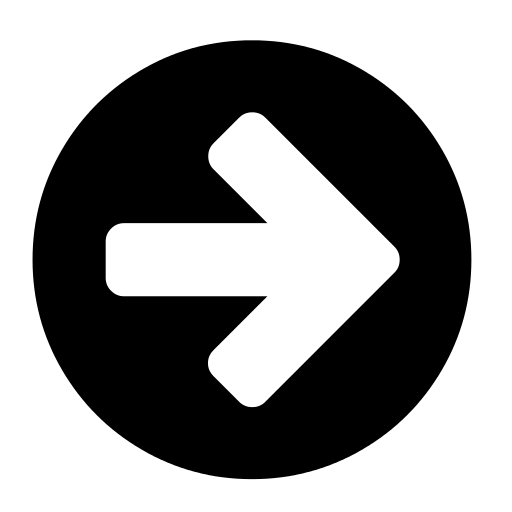
\includegraphics[width=20mm, height=20mm]{./Implementation/Files/arrow.png}
\end{minipage} 	 & \htmlinline{http://commons.wikimedia.org/wiki/File: Circle_arrow_right_font_awesome.svg} \\ \hline

    \begin{minipage}{.5\textwidth}
    
\includegraphics[width=30mm, height=10mm]{./Implementation/Files/volaclogo.jpg}
\end{minipage} 	 & \htmlinline{http://mb.cision.com/Public/3857/ 9287920/93083930d801ade5_800x800ar.jpg} \\ \hline

    \end{tabular}
\end{center}   

\newpage

\section{Code Listing}
\begin{landscape}
%include as many subsections as you have modules
\subsection{Login Window}
%the code below can be uncommented and used to get a code section from a particular file

\pythonfile[firstline=5]{./Implementation/Files/LoginWindow.py}

\newpage
\subsection{Admin Main Program (MainProgram.py)}
\pythonfile[firstline=5]{./Implementation/Files/MainProgram.py}

\newpage
\subsection{Admin Main Menu (AdminMainMenu.py)}
\pythonfile[firstline=5]{./Implementation/Files/AdminMainMenu.py}

\newpage
\subsection{Admin Database Interface (OpenDatabaseWindow.py)}
\pythonfile[firstline=5]{./Implementation/Files/OpenDatabaseWindow.py}

\newpage
\subsection{Admin Search Staff Interface (SearchStaffAdmin.py)}
\pythonfile[firstline=5]{./Implementation/Files/SearchStaffAdmin.py}

\newpage
\subsection{Add Data Window (AddDataGUI.py)}
\pythonfile[firstline=5]{./Implementation/Files/AddDataGUI.py}

\newpage
\subsection{Admin Menubar (MenuBarAdmin.py)}
\pythonfile[firstline=5]{./Implementation/Files/MenuBarAdmin.py}

\newpage
\subsection{Staff Interface (StaffProgram.py)}
\pythonfile[firstline=5]{./Implementation/Files/StaffProgram.py}

\newpage
\subsection{Staff Menu Bar (StaffMenuBar.py)}
\pythonfile[firstline=5]{./Implementation/Files/StaffMenuBar.py}

\newpage
\subsection{Manager Main Program (ManagerMainProgram.py)}
\pythonfile[firstline=5]{./Implementation/Files/ManagerMainProgram.py}

\newpage
\subsection{Department Information Interface (DepartmentInformation.py)}
\pythonfile[firstline=5]{./Implementation/Files/DepartmentInformation.py}

\newpage
\subsection{Manager - My Information (MyInformation.py)}
\pythonfile[firstline=5]{./Implementation/Files/MyInformation.py}

\newpage
\subsection{Manager Menubar (ManagerMenuBar.py)}
\pythonfile[firstline=5]{./Implementation/Files/ManagerMenuBar.py}

\newpage
\subsection{Forgotten Account Interface (ForgottenAccount.py)}
\pythonfile[firstline=5]{./Implementation/Files/ForgottenAccount.py}

\newpage
\subsection{Graph Creation (Graph.py)}
\pythonfile[firstline=5]{./Implementation/Files/Graph.py}

\newpage
\subsection{Dialog Warning Box (PopupDialog.py)}
\pythonfile[firstline=5]{./Implementation/Files/PopupDialog.py}

\newpage
\subsection{Calendar (Calender.py)}
\pythonfile[firstline=5]{./Implementation/Files/Calender.py}

\newpage
\subsection{Confirm Deletion Dialog (ConfirmDialog.py)}
\pythonfile[firstline=5]{./Implementation/Files/ConfirmDialog.py}

\newpage
\subsection{Report Data Error (Reporterror.py)}
\pythonfile[firstline=5]{./Implementation/Files/Reporterror.py}

\newpage
\subsection{Report Bug (BugReport.py)}
\pythonfile[firstline=5]{./Implementation/Files/BugReport.py}

\newpage
\subsection{Login Window (LoginWindow.py)}
\pythonfile[firstline=5]{./Implementation/Files/LoginWindow.py}

\newpage
\subsection{Add Account Interface (AddingAccounts.py)}
\pythonfile[firstline=5]{./Implementation/Files/AddingAccounts.py}

\newpage
\subsection{Change Password Interface (ChangePassword.py)}
\pythonfile[firstline=5]{./Implementation/Files/ChangePassword.py}


\end{landscape}
